\documentclass{standalone}
\usepackage{tikz}
\begin{document}

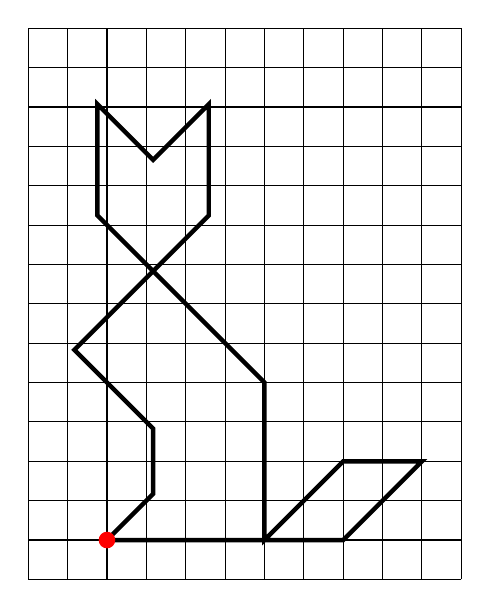
\begin{tikzpicture}
\draw[step=5mm] (-1.0, -0.5) grid (4.5, 6.5);
\draw[ultra thick]
    ({2-3/2*sqrt(2)}, {2+5/2*sqrt(2)}) --
    ({2-sqrt(2)}, {2+2*sqrt(2)}) --
    ({2-1/2*sqrt(2)}, {2+5/2*sqrt(2)}) --
    ({2-1/2*sqrt(2)}, {2+3/2*sqrt(2)}) --
    ({2-sqrt(2)}, {2+sqrt(2)}) --
    ({2}, {2}) --
    ({2}, {0}) --
    ({3}, {1}) --
    ({4}, {1}) --
    ({3}, {0}) --
    ({0}, {0}) --
    ({2-sqrt(2)}, {2-sqrt(2)}) --
    ({2-sqrt(2)}, {sqrt(2)}) --
    ({1-sqrt(2)}, {1+sqrt(2)}) --
    ({2-sqrt(2)}, {2+sqrt(2)}) --
    ({2-3/2*sqrt(2)}, {2+3/2*sqrt(2)}) -- cycle;
\fill[red] (0,0) circle (3pt);
\end{tikzpicture}

\end{document}